\section{Tijdsdilatatie door relatieve beweging}

Beschouw eerst de tijdsdilatatie voor een deeltje dat met hoge snelheid beweegt ten opzichte van het æther-rustframe. Empirisch weten we dat een klok die met snelheid $v$ beweegt, tijd ervaart die langzamer is met de Lorentz-factor $\gamma = 1/\sqrt{1 - v^2/c^2}$. In dit model leiden we hetzelfde effect af door de invloed van absolute æther-beweging op de rotatie van de wervelkern te analyseren.

\subsection*{(a) Kinematische afleiding}

Laat een wervel in rust zijn in zijn eigen frame $S'$ maar met snelheid $v$ bewegen ten opzichte van het æther-rustframe $S$. In $S'$ roteert de wervel met hoekfrequentie $\omega_0$ en definieert de juiste tijd $\tau$. Door Lorentz-tijdsdilatatie ziet een waarnemer in $S$ de klok vertragen:

\begin{figure}[htbp]
    \centering
    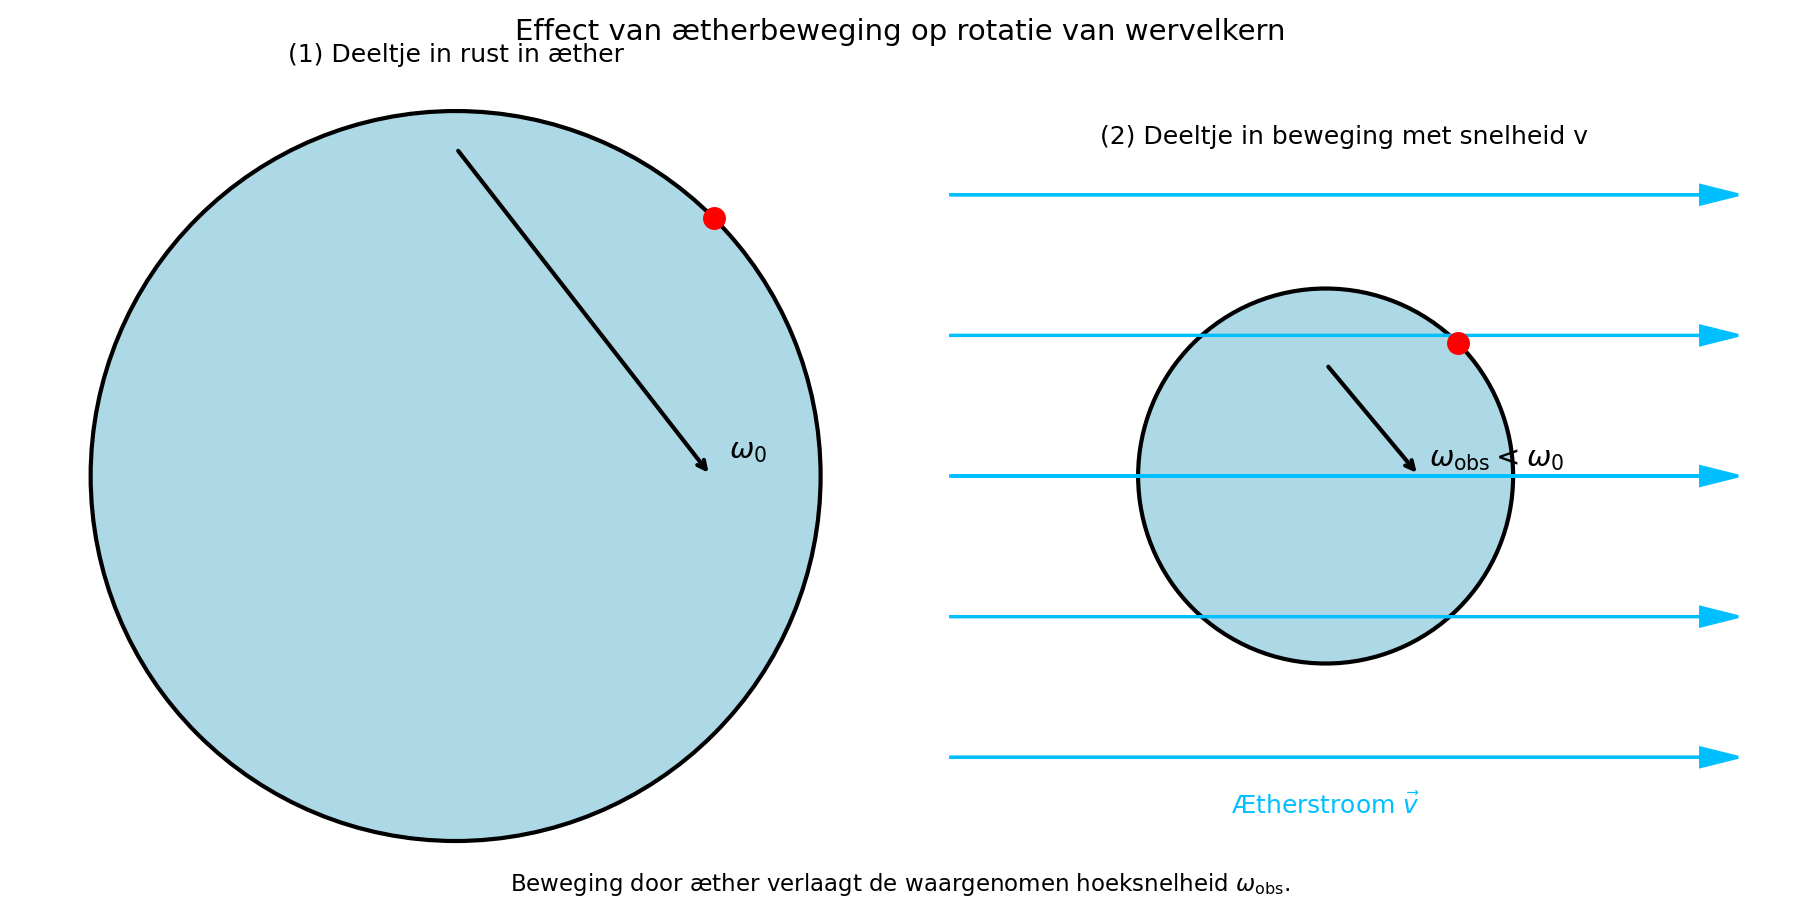
\includegraphics[width=0.85\textwidth]{3-TijdsdilatatieBeweging}
    \caption{Effect van ætherstroming op de interne rotatiesnelheid van een vortexdeeltje. In rust (links) behoudt de wervel zijn maximale hoeksnelheid~$\omega_0$. Bij beweging door de æther (rechts) veroorzaakt de stroming een afname tot~$\omega_{\mathrm{obs}} < \omega_0$.}
    \label{fig:TijdsdilatatieBeweging}
\end{figure}

\[
    \omega_{\text{obs}} = \omega_0 \sqrt{1 - \frac{v^2}{c^2}} \,.
\]
Vanuit de relatie tussen eigentijd en coördinatentijd,
\[
    \frac{d\tau}{dt} = \frac{\omega_{\text{obs}}}{\omega_0} = \sqrt{1 - \frac{v^2}{c^2}} \,. \tag{2}
\]

Dit komt overeen met de standaard SR-tijdsdilatatieformule. In ons model is het fysieke mechanisme dat ætherbeweging over de wervel de wervelsnelheid verstoort, waardoor de schijnbare rotatie in het ætherframe wordt vertraagd.

\subsection*{(b) Vloeistofdynamische interpretatie}

Een complementaire interpretatie gebruikt analogieën van samendrukbare stroming. In de vloeistofdynamica ervaart een lichaam dat met snelheid $v$ beweegt in een samendrukbaar medium met signaalsnelheid $c$ vervormingen evenredig aan $\gamma = 1/\sqrt{1 - v^2/c^2}$. Dit kan worden gezien als een Doppler-tijdsdilatatie of weerstand tegen het handhaven van coherente circulatie.

Naarmate de snelheid de æthersignaalsnelheid $c$ nadert, comprimeert de omringende stroming en biedt weerstand aan wervelrotatie. Daarom daalt de hoeksnelheid die in het ætherframe wordt gezien, en:
\[
    \omega_{\text{obs}} = \omega_0 \sqrt{1 - \frac{v^2}{c^2}} \Rightarrow \frac{d\tau}{dt} = \sqrt{1 - \frac{v^2}{c^2}} \,. \tag{3}
\]

\subsection*{Implication}

Dit geeft ons de relativistische tijdsdilatatie voor een bewegende klok:
\[
    \boxed{\frac{d\tau}{dt} = \sqrt{1 - \frac{v^2}{c^2}}}
\]
binnen een Euclidische, æther-gebaseerde vlakke ruimte, en komt overeen met alle speciale relativiteitstheorie-experimentele voorspellingen~\cite{Rado2020-aether-Lorentz,Levy2009-aether-clock}.